\documentclass[10pt]{beamer}

\usepackage{graphicx}
\usepackage{minted}
\usepackage{proof}
\usepackage{booktabs}
\usepackage[scale=2]{ccicons}

\usetheme[everytitleformat=regular, progressbar=foot]{m}
\usefonttheme[onlymath]{serif}

% Macros
\let\oldemptyset\emptyset
\let\emptyset\varnothing
\newcommand{\case}{\text{ case }}
\newcommand{\of}{\text{of }}
\newcommand{\yields}{\multimap}


\title{Formalising a language with uniqueness typing}
\author{Michael Sproul}
\date{}
\institute{
    Supervisor: Ben Lippmeier\\
    University of New South Wales
}

\begin{document}

\maketitle

\section{Introduction}

\begin{frame}{What?}

\begin{enumerate}
\item Define the \textit{type system} and \textit{semantics} for a small programming language as a formal mathematical system.
\item Prove that the programming language is ``well-behaved" -- \textit{sound}.
\end{enumerate}
\end{frame}

\begin{frame}
{Motivation}

Programming languages are complicated, lots of interacting features.

We want to:

\begin{itemize}
\item Eliminate or minimise undefined behaviour.

% Do closures work well with exceptions?
\item Ensure that language features interoperate without creating unsoundness.

\item Provide a solid foundation for software verification.

\end{itemize}
\end{frame}

\begin{frame}
{Motivation}

Formalised language semantics are a prerequisite for:

\begin{itemize}
\item Proofs about programs. \textit{seL4}, verified crypto.
    \begin{itemize}
    \item Security, correctness.
    \end{itemize}
\item Trust-worthy compilers. \textit{CompCert}.
\item Sanity whilst programming?
\end{itemize}
\end{frame}

\section{Background}

\begin{frame}{Contraction and Weakening}

In regular* logic there are two rules that allow assumptions to be discarded, or introduced from nowhere:

$$
\infer[Contraction]{\Gamma, A \vdash B}{
	\Gamma, A, A \vdash B
}
\qquad
\infer[Weakening]{\Gamma, A \vdash B}{
    \Gamma \vdash B
}
$$

*regular = classical/intuitionistic/constructive

\end{frame}

\begin{frame}{Contraction and Weakening}

Every logic corresponds to a type system, so we have...

\begin{eqnarray*}
\infer[Contraction]{\Gamma, x : A \vdash u[x/y, x/z] :: B}{
	\Gamma, y : A, z : A \vdash u :: B
}
\qquad
\infer[Weakening]{\Gamma, x : A \vdash y :: B}{
    \Gamma\vdash y :: B
}
\end{eqnarray*}

Without contraction, variables can only appear once in a term.
% Note: This is because concatenation of environments requires distinct variables.

Without weakening, all variables in the context must be used in the term.

[Wadler 1991, 1993]

\end{frame}

\begin{frame}{Linear and affine type systems}

\begin{itemize}
\item \textbf{Linear type system:} Contraction and weakening banned -- every value used \textit{exactly} once.
\item \textbf{Affine type system:} Contraction banned, weakening allowed -- every value used \textit{at most} once.
\end{itemize}

From linear logic [Girard 1987] and affine logic [Grishin 1974] respectively.

\end{frame}

\begin{frame}{Retaining intuitionistic behaviour}

Linear type systems allow some terms to be treated in the normal intuitionistic way, via the bang operator, (!).

\begin{eqnarray*}
\emptyset \vdash \lambda \langle x' \rangle . \case x' \of !x \rightarrow \langle !x, !x \rangle :\text{ } !A \yields (!A \otimes !A)
\end{eqnarray*}

Derivable using a version of contraction that requires \textit{non-linear} assumptions [Wadler 1993].
% Talk note: The case statement is required to coerce an assumption of the form x': !A to [x: A].

\end{frame}

\begin{frame}

\frametitle{Why bother?}

Several languages use type systems based on linear logic to provide useful features:

Mutation without sacrificing referential transparency (Clean).



% Talk: Unique references to memory permit destructive updates.


\end{frame}

\begin{frame}[fragile]{Why bother?}

Memory safety without garbage collection -- Cyclone, Rust.

\begin{verbatim}
fn main() {
    // Heap allocated vector - but we don't need to free it!
    let mut v = Vec::new();

    for i in 0 .. 200 {
        v.push(i * i);
    }

    println!("{:?}", v);
}
\end{verbatim}

\end{frame}

\begin{frame}{Uniqueness typing}

Linear (and affine) typing aren't quite enough to guarantee unique references to values.

\textit{Dereliction} allows a non-linear value to be used as a linear one.

In a pure linear (or affine) type system, uniqueness of linear values therefore isn't guaranteed [de Vries 2008].
\end{frame}

\begin{frame}{Uniqueness typing}

\begin{itemize}
\item \textbf{Linear/affine typing}: Linear values \textit{will not} be duplicated at any point in the future.
\item \textbf{Uniqueness typing}: Linear values \textit{have not} been duplicated at any point in the past.
\end{itemize}

\end{frame}

\begin{frame}{Uniqueness typing via attributes}

Edsko de Vries designed a system that uses a uniqueness \textit{kind}, and a type constructor \texttt{Attr} which annotates a type as either unique or non-unique.

\begin{figure}[h]
\centering
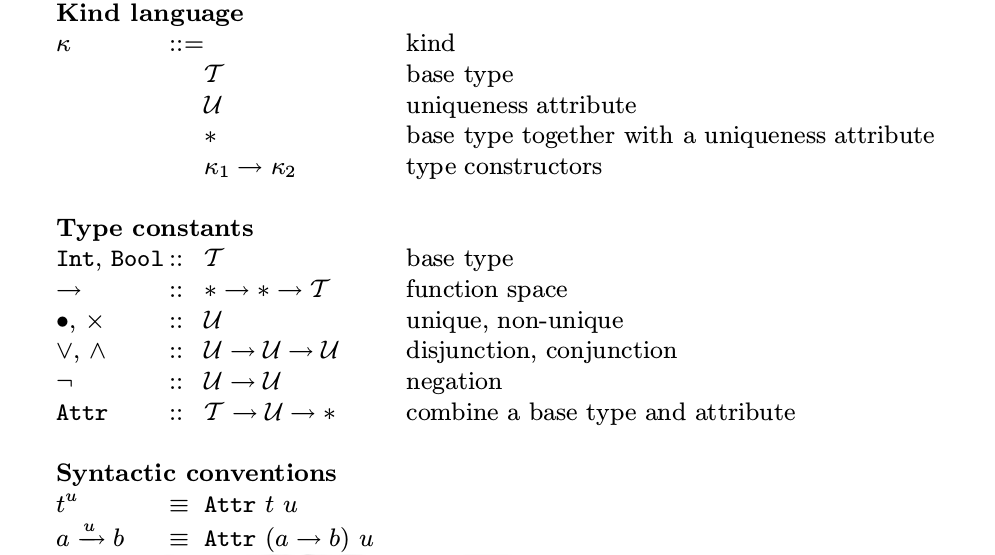
\includegraphics[width=300px]{de_Vries_attributes.png}
\label{}
\end{figure}
% Levity polymorphism?
\end{frame}

\begin{frame}{Uniqueness typing formalisation}
de Vries used Coq to prove soundness for his attribute-based type system.

\begin{itemize}
\item ``Locally nameless" approach to variable naming -- de Bruijn indices for bound variables and names for free variables.\\

\textit{The use of the locally nameless approach, and in particular the use of the Formal Metatheory library, meant that little of our subject reduction
proof needs to be concerned with alpha-equivalence or freshness.}

\end{itemize}
\end{frame}

\begin{frame}{The \textbf{$L^3$} language}
It's great.
% Talk about capabilities.
% Can we do files easily with an extension?
% Time plan (including software foundations).
% Time for pre-research, time for proving, write ups.
% Related work at the very end.
% Francois Potier's stuff (capabilties + uniqueness, frame rule + inverse frame rule JFP). Language: Mezzo.
\end{frame}

\section{Proposal}

\begin{frame}{Proposal}

Define operational semantics and typing rules for a variant of the lambda calculus with \textit{linear} typing, in Coq, using de Bruijn indices for naming.

Prove \textit{progress} and \textit{preservation}.
\end{frame}

\begin{frame}{Progress}

If a term is well-typed, it is either a value, or it can take a step.

[[formal definition here (gotta workout Latex natural deduction)]]
\end{frame}

\begin{frame}{Preservation}

If a term is well-typed and it takes a step, it retains the same type.

\end{frame}

\end{document}
